\pagebreak
\thispagestyle{empty}
\movetoevenpage
\begin{figure}
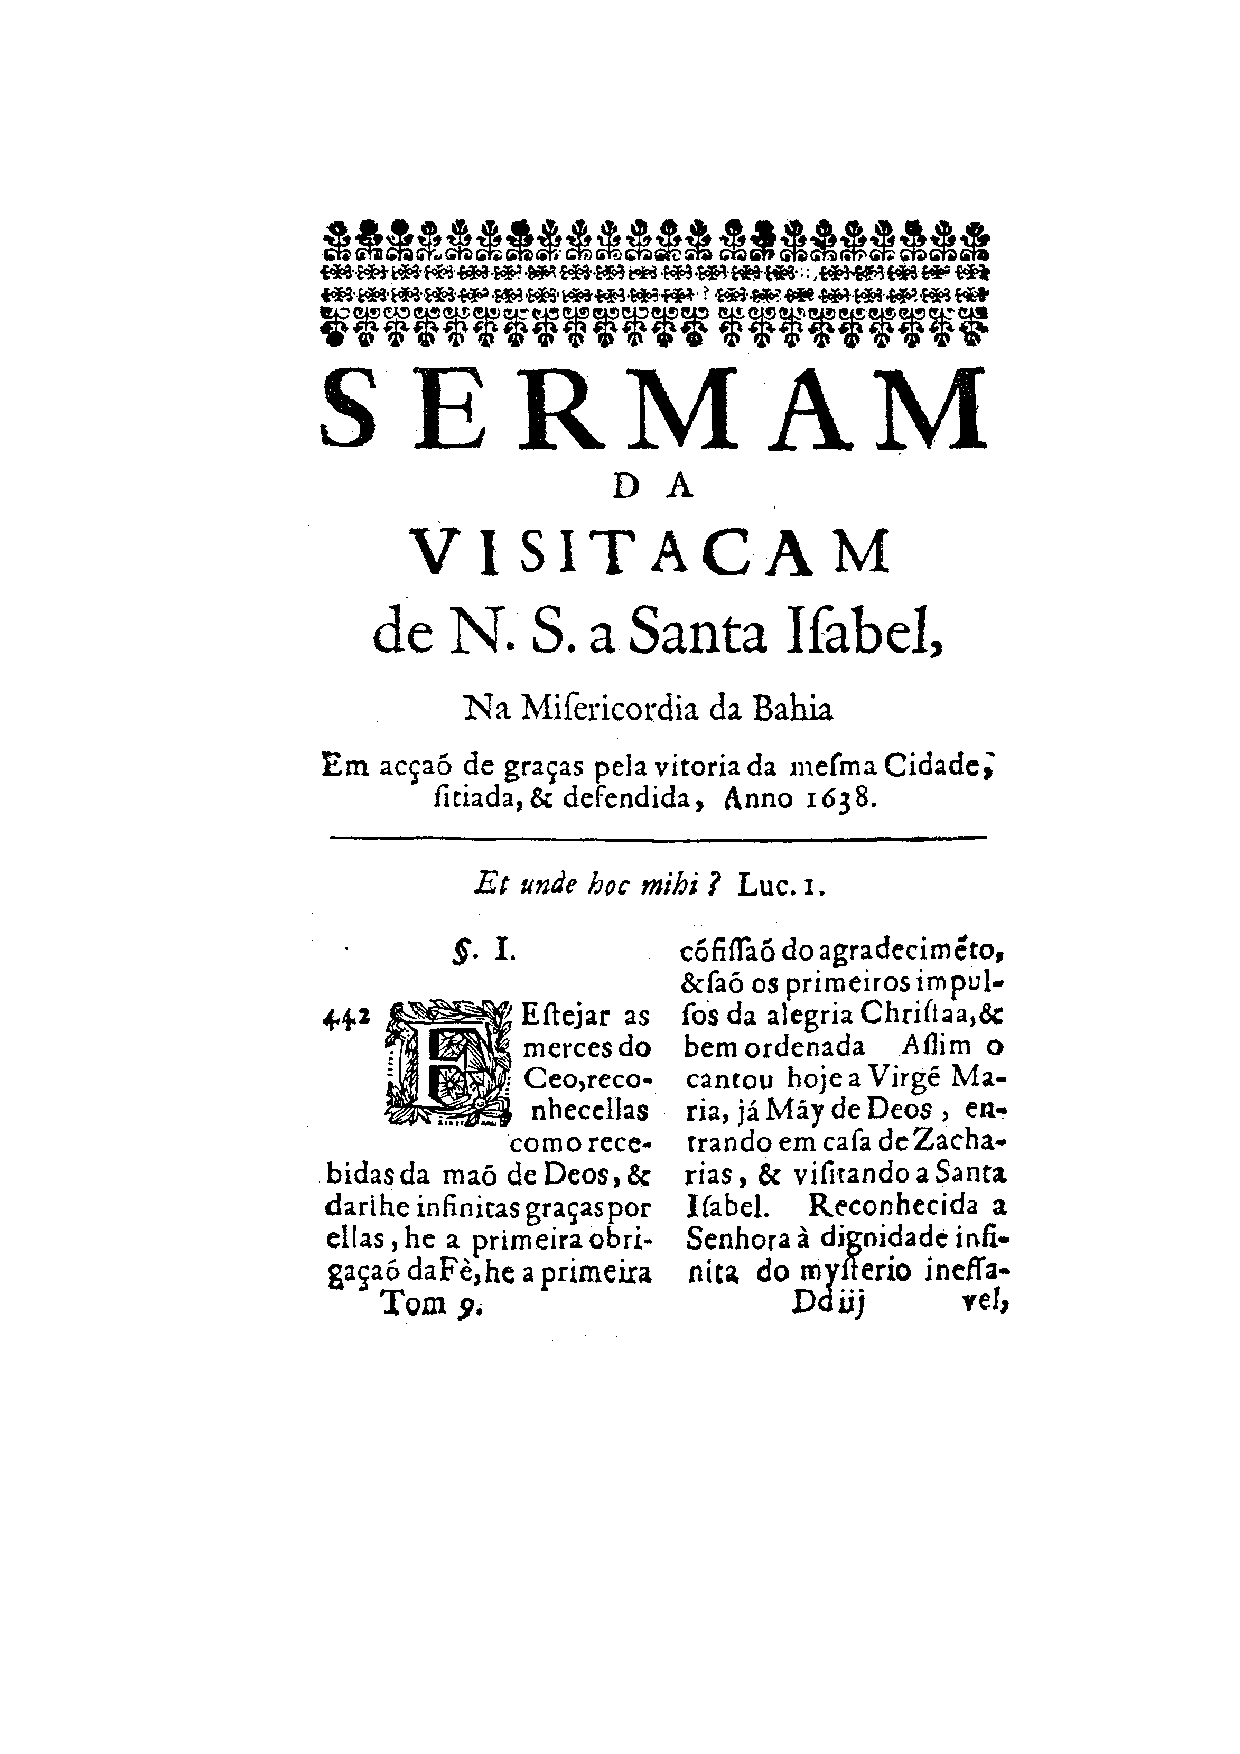
\includegraphics[width=\textwidth]{./imgs/visitacao.pdf}  
\end{figure}

\chapter[Sermão da Visitação de Nossa Senhora a Santa Isabel]{Sermão da Visitação de Nossa\\ Senhora a Santa Isabel}
\hedramarkboth{Sermão da Visitação\ldots{}}{}

\begin{quotation}
\noindent{}Na misericórdia da Bahia,
Em ação de graças pela vitória da mesma Cidade,
sitiada e defendida, Ano 1638.
\end{quotation}

\epigraph{\emph{Et unde hoc mihi?}}{Lc, 1.\footnotemark}\footnotetext{Lc 1[:43] [\textit{E donde a mim esta} dita, que a mãe do meu Senhor venha ter comigo?]}

\section*{I}

\noindent{}Festejar as mercês do céu, reconhecê"-las como recebidas da mão de Deus,
e dar"-lhe infinitas graças por elas, é a primeira obrigação da fé, é a
primeira confissão do agradecimento, e são os primeiros impulsos da
alegria cristã e bem ordenada. Assim o cantou hoje a Virgem Maria, já
Mãe de Deus, entrando em casa de Zacarias, e visitando a Santa Isabel.
Reconhecida a Senhora à dignidade infinita do mistério inefável, que a
mesma Isabel, por revelação do céu, também reconhecia e celebrava, que
fez e disse? Louvou e magnificou a Deus: \emph{Magnificat anima mea
Dominum}:\footnote{Lc 1:46 [Disse, então, Maria: \textit{A minha alma engrandece ao Senhor}.]} alegrou"-se no interior do seu espírito, com
demonstrações semelhantes às do Batista no ventre da mãe:
\emph{Exultavit spiritus meus in Deo salutari meo}:\footnote{Lc 1:47 [E \textit{o meu espírito se alegra em Deus, meu Salvador}.]} e declarou e
confessou que as grandezas, que já começavam a sair à luz, nascidas do
que dentro em si trazia, eram obra do braço todo"-poderoso do Senhor, e
seu santo nome: \emph{Quia fecit mihi magna qui potens est, et santum
nomen ejus}.\footnote{Lc 1:49 [\textit{Porque me fez grandes coisas o Poderoso; e Santo é o seu nome.}]}

Isto é o que nas grandes mercês do céu deve festejar e reconhecer a fé e
agradecimento humano; mas não basta. E que mais é necessário? É
necessário que, voltando os homens os olhos para a terra, os ponham em
si com verdadeiro conhecimento da própria indignidade, e (porque a
providência divina sempre requer disposição ou cooperação de suas
criaturas, para repartir com elas os tesouros de suas misericórdias)
que considerem todos, e se pergunte cada um à si mesmo, e diga com Santa
Isabel: \emph{Et unde hoc mihi?} E donde a mim tão extraordinária mercê?
Assim o fez também a mesma Virgem Maria, no meio dos mesmos louvores
com que magnificou a Deus, e com que se via magnificada, olhando para si
mesma, como diz, e não achando nem reconhecendo em si outro motivo, outra razão, ou
outro porquê das mesmas grandezas, senão o da sua humildade: \emph{Quia
respexit humilitatem ancillae suae}:\footnote{Lc 1:48 [\textit{Porque atentou na humildade de sua serva}; pois eis que, desde agora, todas as gerações me chamarão bem-aventurada.]} Quer dizer: Vós, ó Isabel,
cheia do Espírito Santo, me apregoais por Mãe de Deus: \emph{Ut venial
Mater Domini mei ad me}:\footnote{Lc 1:43 [E donde a mim esta dita, \textit{que a mãe do meu Senhor venha ter comigo?}]} Vós me chamais bendita entre todas as
mulheres: \emph{Benedicta tu inter mulieres}:\footnote{Lc 1:42 [E exclamou em alta voz, e disse: \textit{Bendita és tu entre as mulheres e bendito é o fruto do teu ventre}.]} e vós me
canonizais por bem"-aventurada nesta vida, porque no resto dela se
cumprirão em mim todas as promessas do anjo: \emph{Et beata, quae
credidisti, quoniam perficientur in te quae dicta sunt tibi a
Domino}.\footnote{Lc 1:45 [\textit{E bem-aventurada tu, que creste, porque se hão de cumprir as coisas que da parte do Senhor te foram ditas.}]} E eu não acho nem vejo em mim senão o que só viu o mesmo
Senhor, pondo os olhos na sua menor escrava: \emph{Respexit humilitatem
ancillae suae}.

Até aqui a famosa história da Visitação da Mãe de Deus à mãe do Batista,
na qual, como em parábola, falei até agora de nós e conosco, posto que o
não parecesse. Duas coisas ponderei nela. A primeira, e que naturalmente
move a todo o homem, é
festejar os seus bens, e se é homem cristão, e com fé, louvar á Deus por
eles, e dar"-lhe as devidas graças. A segunda, não parar neste exterior
da felicidade humana, como se fora fortuna ou caso, mas fazer reflexão
sobre si mesmo, e considerar se acha em si algum fundamento de boas
obras, pelo qual Deus se inclinasse ou se deixasse obrigar a lha
conceder. Já cuido que me tenho explicado. Muitos dias há que esta nossa
cidade festeja a ilustre vitória com que Deus lhe fez mercê de se
defender tão gloriosamente do poder do inimigo comum, com que se viu
sitiada. E não há na mesma cidade templo em que, com universal concurso
e aplausos da piedade cristã e portuguesa, se não tenham rendido as
devidas graças ao soberano autor da liberdade que gozamos. Eu hoje nesta
matéria, tão repetida e tão batida como a mesma cidade, já a pudera
passar em silêncio, e emudecer com Zacarias; mas escolhi antes, porque
a Deus não o cansam os agradecimentos, falar com Isabel.

Das suas palavras escolhi por tema somente as da admiração, com que se
pergunta a si mesma: \emph{Unde hoc mihi?} Não falarei em meu nome, mas
a Bahia será a que se admire da vitória, a que tão pouco costumados
estávamos, e a que se pergunte a si mesma donde lhe veio esta ventura
tão extraordinária e tão nova. A Bahia perguntará o donde, e ouvirá as
opiniões dos que cuidam que a eles se lhes deve a vitória. Eu, depois de
responder a cada um por si; concluirei com a que tenho por mais certa e
verdadeira. Isto é o que ouviremos no discurso do sermão, e desde logo o
que só posso dizer é que, para descobrir e achar o donde, não será
necessário ir buscá"-lo à campanha, nem sair à rua, porque o acharemos
dentro nesta mesma casa, como se fora a de Zacarias. Lá e cá temos
derramando graças a fonte da graça. \emph{Ave Maria.}

\section*{II}

\emph{Et unde hoc mihi?} Esta mercê, este favor, este benefício do céu
tão grande, esta felicidade, de que estive tão duvidosa e agora estou
tão segura, esta vitória tão honrada e tão festejada, e de que tão
desacostumado está o Brasil há tantos anos, donde a mim? \emph{Unde
mihi?} Assim pergunta falando consigo a Bahia, e, admirada da sua
própria fortuna, busca dentro em si a causa dela. Mas vejo que desta
mesma pergunta, que sempre supõe dúvida, se dá ou pode dar por muito
ofendido o valor dos nossos soldados, e por igualmente agravada a
reputação das nossas armas.
\emph{Unde,} donde? E quem há tão cego que o não visse nos relâmpagos do
fogo, quem tão surdo que o não ouvisse nos trovões da artilharia, quem
tão seguro e sem receio, que o não temesse em mil e seiscentos raios
contados, que as batarias furiosas do inimigo choveram sobre a Bahia em
quarenta dias e quarenta noites de sítio? Em outros tantos dias e noites
se formou o dilúvio universal que alagou o mundo, e, assim como então
diz o texto sagrado que, não só da parte combatente se abriram as
cataratas do céu, mas também da parte combatida se romperam as fontes do
abismo, assim nesta inundarão, verdadeiramente de monte a monte, se foi
apertada e pertinaz a força dos combates, não foi menor, antes mais
forte e poderosa, a das resistências, de que enfim se confessou por
vencida a soberba e presunção dos mesmos combatentes, quando a sua, não
retirada, mas manifesta fugida, debaixo da capa da noite, mal lhe cobriu
as espaldas.
A artilharia deixada e carregada nas plataformas, sem retirar o inimigo
uma peça; o pão cozendo"-se nos fornos, as olhas dos soldados ao fogo; as
tendas, as barracas, as armas, a pólvora, tudo desamparado, sem ordem,
no precipício da desesperação, não só temerosa, mas atônita; sobretudo,
o silêncio das caixas e das trombetas, com que tão confiados se tinham
aquartelado, mudo e insensível às nossas sentinelas; isto, assim junto
como por partes, é o que está respondendo e dizendo a brados a Bahia a
quem deve, e donde lhe veio o donde por que pergunta. \emph{Unde,}
donde? Da prudência dos nossos ilustríssimos generais, e da bem
aconselhada dissimulação, mal entendida do vulgo, com que deixaram
marchar sem oposição o inimigo, até o lugar onde estava antevista a sua
ruína. \emph{Unde,} donde? Da bizarra resolução dos nossos mestres de
campo, posto que de três nações diferentes, unidos em tomar o governo
das armas, em que só o império e obediência delas entre os dois generais
esteve duvidoso. \emph{Unde,} donde? Do valor dos nossos famosíssimos
capitães e soldados, que antes de haver trincheiras, eles o foram a
peito descoberto, e, depois de as haver,
dentro, com as próprias granadas e bombas do inimigo, e fora, com a
espada na mão, semearam a campanha de, tantos corpos mortos, para cuja
sepultura pediram tréguas, sementeira de que eles logo colheram o
desengano, e nós, pouco depois, o fruto da vitória.

Assim responde a nossa triunfante milícia à pergunta da Bahia, a qual,
posto que testemunha das suas façanhas, ainda duvidosa, inquire e quer
saber qual fosse verdadeiramente o motivo que Deus da nossa parte
tivesse, e qual mais propriamente o onde donde lhe veio o favor do céu,
que tão repetidamente celebra e festeja, querendo dar a glória a aquela
parte de si mesma, à qual mais própria e mais verdadeiramente se deva.

\section*{III}

Primeiramente, respondendo à resposta de nossos soldados, não direi, bom
licença sua, que é muito própria da arrogância militar, mas não posso
deixar de dizer que igualmente é alheia da fé e piedade cristã. Que diz
a fé? Que Deus é o Senhor dos exércitos, e que dá ou tira a Vitória a
quem é servido, por meio das armas sim, mas sem dependência delas. Em
próprios termos a Sagrada Escritura, como se falara nomeadamente do
nosso caso: \emph{Non salvatur rex per multam virtutem, et gigas non
salvabitur in multitudine virtutis suae}:\footnote{S1 33[32]:16 [\textit{Não há rei que se salve com a grandeza de um exército, nem o homem valente se livra pela muita força.}]} Salvou"-se a
cidade do Salvador do perigo em que se viu tão apertada, mas não foi o
numeroso dos seus presídios, nem o valoroso dos seus soldados o que a
salvou, porque na guerra e nas batalhas nem aos reis os salva o poder
dos seus exércitos: \emph{Non salvatur rex per multam virtutem}, nem
aos gigantes os salvam as desmedidas forças dos seus braços: \emph{Et
gigas non salvabitur in multitudine virtutis suae.}

Ouçam os soldados uma e outra coisa da boca de um também soldado, e
soldado que foi rei, \emph{meo sperabo, et gladius meus non salvabit me}.\footnote{S1 43:7 [\textit{Porque não foi no meu arco que pus confiança, nem foi a minha espada que me salvou.}]}
Eu, diz Davi, nunca pus nem porei a esperança da vitória no
meu arco, nem confiarei que me salvará das mãos de meus inimigos a minha
espada. No arco entendem"-se as armas de longe, na espada as de perto e
em umas e outras parece que experimentou o mesmo Davi o contrário do que
diz, porque no desafio do gigante de longe, com o tiro da funda lhe
meteu a pedra na testa, e de perto, com a espada do mesmo inimigo já
prostrado, lhe cortou a cabeça. Pois, se Davi venceu o gigante com o
tiro da funda e com o talho da espada, como diz que não há de pôr a sua
esperança nem nas armas de longe, nem nas de perto? Porque uma coisa é
vencer por meio das armas, outra é pôr a esperança nelas. Pôr a
esperança nas armas é presunção e vaidade gentílica; pô"-la só em Deus,
que é o Senhor das vitórias, é fé e piedade cristã.
Assim sucedeu no mesmo caso, e o disse o mesmo Davi, respondendo às
arrogâncias do gigante: \emph{Tu venis ad me in gladio, et hasta, et
clypeo: ego autem venio ad te in nomine Domini exercituum}:\footnote{1Rs 17:45 [Mas Davi disse ao filisteu: \textit{Tu vens a mim com espada, lança e escudo; eu,
porém, venho a ti em nome do Senhor dos exércitos}, do Deus das tropas de Israel, as quais tu insultaste hoje.]}
Tu, ó gigante, vens contra mim coberto de ferro, com a espada
cingida, com a lança em uma mão e o escudo na outra; eu venho contra ti
desarmado, mas em nome dos exércitos. E que se seguirá desta batalha tão
desigual? \emph{Et dabit te Dominus in manu mea, et percutiam te, et
auferam capuz tuum a te}:\footnote{1Rs 17:46 [\textit{E o Senhor te entregará nas minhas mãos, e eu te ferirei e te cortarei a cabeça}, e darei hoje às aves do céu e aos animais da terra os cadáveres do acampamento dos filisteus, a fim de que toda a terra saiba que há um Deus em Israel.]} Seguirse"-á que Deus com todas
essas armas te entregará nas minhas mãos, e eu, como me vês, desarmado,
te cortarei a cabeça. E que mais? \emph{Et noverit universa ecclesia
haec, quia non in gladio et basta salvat Dominus: ipsius enim est bellum}:\footnote{1Rs 17:47 [{E para que toda esta multidão conheça que o Senhor não salva pela espada, nem pela lança, porque ele é o Senhor da guerra} e vos entregará nas nossas mãos.]}
E conhecerá todo este imenso teatro dos dois grandes
exércitos postos à vista, que para Deus dar a vitória a uns, e pôr em
fugida a outros, não há mister nem faz caso de armas, porque é Senhor da
guerra.

Não sei se teve Davi pensamento particular em chamar à multidão dos que
o viam e ouviam nomeadamente igreja: \emph{Et noverit universo ecclesia
haec}. Porque a fé daquela doutrina nem pertencia ao gentio, quais eram
os filisteus, nem a reconhece o herege,
quais são os de Holanda (e foram os que lá e cá, desenganados da sua
fraqueza, fugiram), mas só e própria dos filhos da verdadeira Igreja,
quais somos nós os católicos. Por isso Davi não só disse igreja, mas
\emph{universa,} que quer dizer católica: \emph{Et noverit universa
ecclesia.} E para que esta fé e este conhecimento? Para que a fortuna
das nossas armas, posto que vitoriosas, nos não desvaneça, antes temamos
as nossas mesmas vitórias, se, ingratos e infiéis a Deus, as atribuirmos
às nossas armas e ao nosso valor. Detrás da carroça dos triunfadores
romanos era costume ouvir"-se um pregão, que dizia: \emph{Memento te esse
mortalem:} Lembra"-te, ó triunfador, que és mortal. E eu neste mesmo
ponto quero fazer outro memento, e publicar outro pregão aos nossos
capitães e soldados, pregão não decretado no capitólio de Roma, mas no
consistório do Triunvirato divino, e não para nos diminuir a alegria do
presente triunfo, mas para que a moderemos com a razão, e a seguremos
com o temor.

Anunciou o profeta Amós a el"-rei Amasias que de seu exército, que
constava de quatrocentos mil homens, licenciasse e despedisse cem mil,
porque eram de gente que estava fora da graça de Deus (notem as
consciências militares quanto importa estarem em graça de Deus ou fora
dela) e como Amasias reparasse nesta diminuição do seu exército, e no
soldo de cem talentos de prata, com que já os tinha pago, respondeu o
profeta, e declarou ao rei da parte de Deus um segredo, que nem ele
então entendia, professando a verdadeira fé, nem hoje acabam de o
entender os que a professam. Ouvi o segredo e o pregão: \emph{Quod si
putas in robore exercitus bella consistere, supera ri te faciet Deus ab
hostibus. Dei quippe est adjuvare, et in fugam convertere}:\footnote{2Par. 25:8 [\textit{Se julgar que o sucesso da guerra depende da força do exército, Deus fará que sejas vencido pelos inimigos, porque só Deus pode socorrer e pôr em fuga.}]}
Porque hás de saber, ó rei, que se imaginares que os felizes sucessos da
guerra, e as vitórias, consistem no número e fortaleza dos exércitos,
pelo mesmo caso e por esta só imaginação fará Deus que seja vencido de
teus inimigos, para que entenda e se desengane o mundo, que dar a
vitória a uns, ainda que sejam poucos e fracos, e pôr em fugida a
outros, ainda que sejam muitos e fortes, não é consequência das armas e
do valor, mas regalia própria do Senhor dos exércitos. Logo, não foi o
esforço nem a ciência militar dos nossos defensores o onde donde a Bahia
pergunta que lhe veio o bem da vitória que festeja: \emph{Unde hoc
mihi?}

\section*{IV}

A esta primeira resposta, e mais palpável à vista, se segue a
segunda, menos visível, mas muito mais poderosa ainda, que é de mãos
desarmadas. Desarmadas estavam as mãos de Moisés quando ele orava no
monte, e o exército de Josué pelejava na campanha. E foi maravilha então
notada de todos, e cuja memória quis Deus ficasse estampada, não em
lâminas de bronze ou diamante, mas nos caracteres imortais dos seus
livros, que quando Moisés levantava as mãos ao céu, vencia Josué, e
quando elas, como de braços cansados já com a velhice, descaíam um
pouco, prevalecia o inimigo: \emph{Cumque levaret Moyses manus vincebat
Israel: sin autem paululum remisisset, superabat Amalech}.\footnote{Ex 17:11 [E acontecia que, \textit{quando Moisés levantava a sua mão, Israel prevalecia; mas, quando ele abaixava a sua mão, Amaleque prevalecia.}]}
Moisés no monte, Josué no campo raso, ambos assestavam as suas batarias
contra o exército de Amalech; mas as máquinas militares e a pontaria dos
tiros eram muito diversas. Josué batia o inimigo, Moisés batia o céu;
Josué com ferro e fogo, Moisés com as mãos desarmadas; Josué ferindo,
Moisés orando: e a vitória estava tão dependente da oração de um, e tão
pouco sujeita às armas do outro, que estas, sem o socorro da oração,
eram vencidas, e só pela força e perseverança da oração vencedoras.

Lembremo"-nos agora de nós. Quem visse interiormente a Bahia
naqueles quarenta dias e quarenta noites em que esteve sitiada, mais a
julgaria, na contínua oração, por uma Tebaida de anacoretas que por um
povo e comunidade civil, divertida em tantos outros ofícios e
exercícios. Nos conventos religiosos, nas igrejas públicas, nas casas e
famílias particulares, todos oravam. Os pais, os filhos, e quantos
podiam menear as armas, assistiam com Josué na campanha; e as mães, as
filhas, e todo o outro sexo ou idade imbele, orando continuamente pelas
vidas daqueles que por instantes temiam lhes entrassem pelas portas ou
mal feridos ou mortos. O estrondo
das batarias inimigas e nossas, espertando com a evidência e temor
do perigo os ânimos, não lhes permitia quietação nem sossego; e então a
Bahia, como propriamente Bahia de Todos os Santos, invocando a
intercessão e auxílio de todos, não por intervalos, como Moisés, mas
perpetuamente e sem cessar, batia as muralhas do céu.

Esta bataria das mãos desarmadas, mas levantadas ao céu, foi mais
verdadeiramente a que nos deu a vitória. E porque a proposta, como de
quem não professa as armas, não pareça suspeitosa aos professores delas,
ouçamos o testemunho de um soldado, e seja o mesmo que já ouvimos na
resposta passada, Davi. Este grande soldado, como capitão general das
armas católicas daquele tempo, em um salmo que campos estando para sair
em campanha, apontando para os esquadrões do exército contrário, que já
tinha à vista, diz assim: \emph{Hi in curribus, et hi in equis, nos autem in
nomine Dei nostri invocabimus}:\footnote{S1 19:8 [\textit{Estes nas suas carroças, e aqueles nos seus cavalos; nós, porém, somos fortes no nome do Senhor, nosso Deus}.]} A milícia de nossos inimigos e a
nossa, ó companheiros, segue mui diferentes máximas: eles põem o seu
poder e toda a sua confiança na multidão da sua cavalaria e nas máquinas
dos seus carros. Porém, nós, que temos outra fé e outra experiência,
posto que com as armas nas mãos, não pomos a confiança nelas, mas todo o
nervo da nossa guerra consiste em outros instrumentos bélicos, muito
mais fortes, que são as orações e preces com que invocamos a Deus: \emph{Nos
autem in nomine Domini invocabimus}. E cuja será a vitória em tanta
diferença de uns e outros combatentes? Eu vo"-lo direi (diz Davi) antes
da batalha, tanto ao certo como se já tivera sucedido, e não só como
profeta, mas como capitão: \emph{Ipsi obligati sunt, et ceciderunt; nos autem
surreximus; et erecti sumus}.\footnote{S1 19:9 [\textit{Eles vacilaram e caíram, mas nós conservamo-nos de pé, e permanecemos firmes}.]} Eles com as suas armas, estando
levantados, caíram vencidos; nós com as nossas orações, estando caídos,
levantamo"-nos vencedores.

Tudo isto é o que sucedeu na nossa vitória. E se eu me atrevesse a
dizer que o mesmo profeta a anteviu é descreveu tão pontualmente, não
faltará quem me diga que não apaixone tanto por ela, pois tem a objeção
ou réplica muito à flor da terra. O profeta fala de inimigos confiados
na sua cavalaria e carros militares, que são os que a milícia antiga
chamava falcatos, e os nossos inimigos não trouxeram cavalaria nem
carros bélicos para nos sitiar. Mas a diferença desta circunstância não
desfaz a profecia, porque o mesmo profeta, falando das naus e armadas
marítimas, lhes chama cavalos e carros: \emph{Viam fecisti in mari equis ruis,
et quadrigae tuae salvatio}:\footnote{Hab 3:15 [\textit{Tu abriste caminho aos teus cavalos pelo mar}, pelo lodo das águas profundas.]; Hab 3:8 [Porventura é contra os rios, Senhor, que tu estás irado? É contra os rios o teu furor? Ou é contra o mar a tua indignação? Tu, que montas sobre os teus cavalos, e levas \textit{em tuas quadrigas a salvação}.]} e tais foram os cavalos e carros
militares, com que na sua poderosa armada naval nos sitiou por mar o
inimigo: \emph{Hi in curribus, et hi in equis.} Eles, porém, posto que
tão exercitados nesta cavalaria nadante, tendo entrado tão soberbos e
inchados como as suas velas, e tão levantados com os sucessos da passada
fortuna como as suas bandeiras no tope, sendo ainda mais altos os seus
pensamentos, caíram; e nós, posto que verdadeiramente caídos com a
adversidade dos mesmos sucessos, se nos levantamos vencedores e
triunfantes é porque a força da oração, e não a das armas, neste
levantar a cair trocou as balanças de Marte: \emph{Ipsi obligati sunt,
et ceciderunt; nos surreximus, et erecti sumus.}

\section*{V}

Naquela famosa batalha dos troianos contra os latinos, diz o Príncipe
dos poetas que, enquanto a vitória esteve duvidosa, Júpiter sustentava
na mão duas balanças iguais, até que uma caiu vencida, e outra se
levantou vencedora:

\begin{verse}
\emph{Jupiter ipse duas aequato examine lances}\\
\emph{Sustinet, etc.}\footnote{Virgílio. \textit{Eneida}. Canto \textsc{ix}.}
\end{verse}

E Filo Hebreu, prosseguindo a mesma metáfora, não
fabulosa e poeticamente mas fundado na verdade da História Sagrada, diz
que as armas de Josué, como postas em balança, sem a oração de Moisés
caíam, e com a oração de Moisés se levantavam: \emph{Cum igitur
aliquantisper manus, bilancis in morem, nunc sursum tollerentur, nunc
deorsum vergerent, certaretur marte dubio; tandem repente, velut pennas
habentes pro digitis, sublatae volitabant per aerem manentes in sublimi,
donec Hebraeis certa victoria contigit, hostibus internectione deletis.}\footnote{Philo \textit{in} eum locum.}
Notem"-se muito aquelas palavras: \emph{nunc sursum
tollerentur, nunc deorsum vergerent bilancis in morem}: de sorte que a
vitória estava posta na balança da oração, já descendo, já subindo, não
conforme Josué mais ou menos fortemente meneava as
armas, mas segundo as mãos de Moisés, ou orando remissamente
desfaleciam, ou, instantemente levantadas ao céu, como se os seus dedos
fossem asas, voavam: \emph{Velut pennas habentes pro digitis, sublatae
volitabant.}

Daqui se segue que, se a justiça, com as balanças em uma mão e a espada
na outra, houver de julgar a nossa vitória a quem mais verdadeiramente
se deve, não há de ser a espada dos que, como Josué, pelejavam na
campanha, senão as mãos levantadas dos que no mesmo tempo, como Moisés,
oravam no monte. E para que os nossos capitães se não ofendam desta
proposição, e desafiem a quem a quiser sustentar, lembrem"-se que no
antigo povo de Deus, em que houve Josué, Sansão, Gedeão e Davi, o mais
afamado Capitão de todos foi Judas Macabeu, e lembrem"-se também que
entre as mais celebradas e fatais espadas (ainda que entrem nesta conta
as forjadas na oficina de Vulcano, batidas e limadas por Brontes e
Esterope, e caldeadas na lagoa Estígia), nenhuma houve igual à do mesmo
Macabeu, a qual, trazida do céu, e dourada nos resplendores líquidos das
estrelas, lhe entregou a alma do profeta Jeremias. Mas, quais foram os
troféus e triunfos deste Aquiles com tão prodigiosa espada?
É certo, e de fé, que foram tantas as suas vitórias quantas as batalhas,
como se trouxesse a soldo a fortuna debaixo das suas bandeiras; contudo,
depois de tantas vezes vencedor o famoso Macabeu, e de ter conquistado o
glorioso nome de invicto entre todas as nações do mundo, finalmente, na
batalha contra Báquides, tendo triunfado de outro muito maiores
exércitos, foi vencido e modo. E por quê? Porque este valorosíssimo
capitão; ou conquistando, ou defendendo, ou sitiando, ou sendo sitiado,
ou guerreando em campanha aberta; sempre às forças do braço e da espada
ajuntava as da oração, e só nesta última e infeliz batalha (como em
muitos lugares nota A Lápide) não se lê na Escritura que orasse. Tão
fortes e invencíveis são as armas acompanhadas da oração, e tão fracas e
sujeitas a ser vencidas se as não assiste este divino e todo"-poderoso
socorro. Assim que, se a Bahia ainda duvida, e pergunta donde lhe veio a
felicidade da vitória, com que se vê segura e triunfante; \emph{Unde hoc
mihi?} saiba que mais a deve às mãos levantadas que às mãos armadas,
mais aos que batiam o céu que aos que combatiam o inimigo, mais aos que
por ela oravam que aos que pelejavam por ela.

\section*{VI}

Temos respondido à Bahia com duas resoluções, ambas certas, e me detive
tanto na prova de ambas, porque ainda estamos em tempo de as haver
mister. O inimigo, ainda que fraco, nunca se há de desprezar, quanto
mais poderoso! E se é poderoso e afrontado, então se deve temer, e
esperar com maior cautela. Desenganados, pois, no primeiro discurso, que
as vitórias se não devem atribuir só ao valor dos soldados e força das
armas, e persuadidos no segundo, que antes se deve esta glória à
eficácia e socorro das orações, com que a nossa defesa de dia e de
noite, pública e privadamente, foi tão assistida, agora quero eu
declarar o meu pensamento, e peço que, antes de ouvido os fundamentos
dele, mo não estranhem ou condenem.

Respondendo, pois, terceira vez absoluta e resolutamente à pergunta da
Bahia: \emph{Unde hoc mihi?} Digo que o donde lhe veio a vitória que
celebra é desta mesma Casa de Misericórdia em que estamos, e que os
soldados, aos quais principalmente se deve, são os que militam debaixo
da sua bandeira. Os que militam debaixo da bandeira da misericórdia, por
diverso modo, ou são os irmãos, que exercitam as obras da mesma
misericórdia com os pobres e enfermos, ou são os mesmos pobres e
enfermos, que eles sustentam, remedeiam e curam; e, posto que estes
pareçam incapazes de pelejar, a uns e outros se deve igualmente a
gloriosa defensa da nossa metrópole.
Tudo isto provará em seu lugar o nosso discurso.

\emph{Beatus qui intelligit super egenum et pauperem}.\footnote{S1 40:1 [\textit{Bem-aventurado o que cuida do necessitado e do pobre}; o Senhor o salvará no dia mau.]} Ditoso e bem"-aventurado,
diz o profeta rei, todo aquele que entende e se ocupa em servir e
remediar os pobres. Não é este o fim e instituto da santa Irmandade
da Misericórdia, como se foram as palavras tresladadas do seu próprio
compromisso? Sim. E por que diz o profeta que são ditosos e
bem"-aventurados todos os que se exercitam e ocupam em obra tão pia?
Segue"-se o porquê: \emph{In die mala liberabit eum Dominus}.\footnote{S1 40:1 [Bem-aventurado o que cuida do necessitado e do pobre; \textit{o Senhor o salvará no dia mau}.]}
Porque no dia mau, isto é, nas ocasiões de aperto e perigo, os
livrará Deus; e se o perigo e aperto for de guerra, em que se virem
acometidos, sitiados ou assaltados, Deus não permitirá que sejam
entregues ao poder de seus inimigos: \emph{Et non tradet eum in animam
inimicorum ejus}.\footnote{S1 40:3 [O Senhor o guardará e lhe conservará a vida, e o fará feliz na Terra, \textit{e não o entregará ao desejo dos seus inimigos}.]} Note"-se a palavra \emph{in animam}. O ânimo
com que vinha o inimigo era de que a Bahia se lhe entregasse
(oferecimento que tantas vezes nos fez pelos seus trombetas) e, por
consequência, se lhe rendesse o resto do Brasil. Mas Deus lhe
desanimou esse ânimo, e lho desmaiou de tal maneira, como mostrou o
sucesso.

E por que não pareça que esta promessa divina, de defender aos que se
ocupam no remédio é cura dos pobres, é só feita a eles, é digna de se
não passar em silêncio uma sutileza de Hugo Cardeal, sobre as palavras:
\emph{Dominus conservet eum},\footnote{S1 40:3 [\textit{O Senhor o guardará} e lhe conservará a vida, e o fará feliz na Terra, e não o entregará ao desejo dos seus inimigos.]} que se seguem no mesmo texto:
\emph{Conservet eum}, diz o grande comentador, \emph{id est, cum aliis
servet.} O verbo simples, \emph{servare,} significa guardar e defender
absolutamente; o composto, \emph{conservare,} por virtude ou aditamento
daquela preposição com, não só significa guardar e defender de qualquer
modo, senão guardar e defender"-se a si com outros, ou a outros consigo:
\emph{Conservet eum, id est, cum aliis servet.} Explico e aplico
juntamente, por não gastar dois tempos. Assim como uma cidadela muito
forte, não só defende aos que estão dentro, senão aos de toda a cidade,
assim esta Casa da Misericórdia (por isso, não acaso, senão com grande
providência, levantada e colocada no coração da Bahia) não só guardou e
defendeu aos da mesma casa, que são os que nela exercitam as obras de
misericórdia, senão a todos os mais. É o que já tinha dito com o mesmo
pensamento Santo Agostinho: \emph{Deus, qui habitat in vobis, custodiet
vos ex vobis, id est, si alter solicitus ex altero}.\footnote{Aug. in regula c1ericorum [PL: Vol. 32: \textit{Opera Omnia Augustini Hipponensis}. S. Augustini Tomus Primus. Augustinus Hipponensis: S. Aurelii Augustini Hipponensis Episcopi Regula ad Servos Dei. Regula. De habitu et exterioris hominis compositione.]} Quando vós
fordes solícitos, e procurardes o bem e saúde uns dos outros, Deus, que
habita em vós, guardará também a uns pelos outros, isto é, \emph{vos ex
vobis}, vós que não tendes essa ocupação nem esse cuidado, pelos que o
têm.
Quem tem o cuidado dos pobres: \emph{Qui intelligit super egenum et
pauperem?} Os que curam deles, e os servem nesta Casa de Misericórdia; pois vós, os
que não sois da mesma casa, e não professais ser Irmãos da Misericórdia,
também vós sereis guardados e defendidos, não por vós, senão por eles:
\emph{Vos ex vobis.} Só apontando com o dedo se pode isto declarar.
Vós, que não sois Irmãos da Misericórdia, por benefício e merecimento de
vós, que o sois: \emph{Vos ex vobis.}

\section*{VII}

Já temos o primeiro e principal fundamento da nossa felicidade, que foi
livrar"-nos Deus do poder e intentos do inimigo: \emph{In die mala
liberabit eum Dominus, et non tradet eum in animam inimicorum
suorum}. Passemos agora ao glorioso da vitória, sem nos
apartar em nada, antes confirmando em tudo a verdadeira causa dele.
Entrou Cristo, Redentor nosso, triunfando em Jerusalém, e os que
acompanhavam e seguiam o triunfo com aclamações e aplausos:
\emph{Caedebant ramos de arboribus}:\footnote{Mt 21:8 [E muitíssima gente estendia as suas vestes pelo caminho, e outros \textit{cortavam ramos de árvores} e os espalhavam pelo caminho.]} cortavam ramos das
árvores, diz o evangelista, e estes ramos, como declara o uso e
tradição da Igreja, e refere o antiquíssimo Clemente
Alexandrino,\footnote{Clemens, lib. 1, paedag., cap. 5.} eram de oliveira e palma. Não pare o
triunfo, mas reparemos nós na união destes ramos. Os ramos da palma
muito bem diziam com o triunfo, porque cada folha dos ramos das palmas é
uma espada; porém a oliveira, que antes significa paz que guerra,
misericórdia e piedade, e não violência nem rigor, por que se ajunta
neste triunfo com a palma?
Por isso mesmo. Porque a palma significa a vitória, a oliveira significa
a misericórdia, e nos triunfos dos cristãos, como no de Cristo, os ramos
da palma andam tão unidos, e como enxertados nos da oliveira, que da
oliveira dependem as palmas, e da misericórdia as vitórias. Drogo
Hostiense: \emph{Egredere cum pueris Hebraeis, qui transeunt,simpliciter
in occursum Domini, sterne in via ramos olivarum, et opera misericordiae
pedibus ejus accommoda: accipe frondes palmarum, ut triumphes}.\footnote{Drog. de Passo Sacram. [\textit{PL}: Vol. 166: Anna Domini \textsc{mcxxxvii} et \textsc{mcxxxiiii} Drogo Cardinalis Astiensis Episcopus. Drogo Cardinalis: Drogonis Cardinalis Sermo de Sacramento Dominicae Passionis. (Biblioth. Patr. Lugdun., \textsc{xxi}, 329.)]}
Se quereis vitórias, soldados de Cristo, não vos digo que imiteis os
Sansões, nem os Gedeões dos hebreus, senão a simplicidade dos meninos de
Jerusalém. E como? Diz à evangelista que os meninos lançavam os ramos no
caminho por onde o Senhor triunfante havia de passar: \emph{Sternebant
in via}:\footnote{Mt 21:8 [E muitíssima gente estendia as suas vestes pelo caminho, e outros cortavam ramos de árvores e os \textit{espalhavam pelo caminho}.]} e vós da mesma maneira os ramos da oliveira, que
são as obras de misericórdia, aplicai"-as aos pés de Cristo, que são no
seu corpo místico os pobres e miseráveis: \emph{Et opera misericordiae
pedibus ejus accommoda}: e logo tomai e levantai os ramos das palmas
vitoriosas, porque sem dúvida triunfareis: \emph{Accipe frondes
palmarum; ut triumphes.}

Já veríeis a imagem da vitória armada, e com a espada em uma mão e a
palma na outra; eu quero emendar esta imagem, porque mais parece
gentílica que cristã.
Aceito a palma em uma mão, e por que se não queixem os soldados, também
a espada na outra; mas ainda lhe falta a esta pintura a principal
insígnia da vitória. E qual é? A Coroa. \emph{Non coronabitur nisi qui
legitime certaverit}:\footnote{2Tm 2:5 [E, se alguém também milita, \textit{não é coroado se não militar legitimamente}.]} Não será coroado como vencedor,
senão o que pelejar legitimamente. Entre os romanos havia grande
multidão e variedade de coroas: cívicas, murais, rostratas, castrenses,
etc., e as principais eram formadas de ervas e plantas, como também as
dos imperadores, porque naquele tempo coroava"-se a honra, e não a
cobiça. De que há de ser pois formada ou tecida esta coroa da imagem da
vitória emendada? Digo que há de ser tecida de ramos de oliveira, e de
oliveira sinaladamente, porque a oliveira é símbolo da misericórdia e
das obras dela. Ouvi um grande texto. Davi era tão piedoso e compassivo
como valente: virtudes que sempre andam juntas, assim como a crueldade é
própria dos covardes e fracos. E falando aquele grande capitão com a sua
alma (com a qual os que seguem as armas costumam ter pouca conversação)
diz"-lhe assim: \emph{Benedic, anima mea, Domino, et noli oblivisci
omnes retributiones ejus, qui propitiatur omnibus iniquitatibus tuis,
qui redimit de interitu vitam tuam, qui coronat te in misericordia et
miserationibus}:\footnote{S1 102:2--4 [\textit{Bendize, ó minha alma, o Senhor, e não esqueças nenhum de seus benefícios}. É ele \textit{quem perdoa todas as tuas culpas}, e que sara todas as tuas enfermidades. É ele \textit{quem resgata da morte a tua vida}, e \textit{que te coroa de misericórdia e de graça}.]}
Louva, alma minha, a Deus, e não te esqueças das grandes mercês que tens
recebido de sua liberal e poderosa mão. Lembra"-te que ele é que te tem
perdoado os teus pecados, ele o que na guerra te livrou tantas vezes a
vida, e ele o que te coroou nas vitórias com a misericórdia e suas
obras; isso quer dizer: \emph{in misericordia et miseratianibus:
misericordia in habitu, miserationibus in effectu.}\footnote{Hugo ibi.} E cuja foi esta
misericórdia que coroou a Davi vitorioso? Foi a misericórdia de Deus,
que por sua misericórdia o coroou, ou foi a misericórdia de Davi, o qual
nela deu a matéria a Deus para o coroar? Responde Dídimo, antigo padre
grego, esquisita e finamente que a misericórdia e obras de misericórdia
de Davi foram a matéria de que Deus lhe teceu a coroa com que o coroou:
\emph{Coronat te in misericordia et miserationibus, quippe coronae
materia est misericordia et miseratio; sicut enim alii coronam justitiae
percipiunt ex justitia contextam, sic etiam tu, o anima mea, ex
misericordia et miserationibus coronaberis}.\footnote{Didym. Ibi in Caena Graecor \textsc{pp}.} Notem"-se muito
aquelas grandes palavras: \emph{quippe coronae materia est misericordia
et miseratio.} De sorte que a matéria, de que foi formada e tecida por
Deus a coroa de Davi vitorioso, foi a misericórdia e obras de
misericórdia do mesmo Davi. E como a misericórdia em divinas e humanas
letras é simbolizada na oliveira, de oliveira há de ser a coroa que na
imagem ou estátua da Vitória emendada se lhe há de acrescentar à palma.

\section*{VIII}

Agora se segue o que parece mais dificultoso na minha proposta, e é
dever"-se a nossa vitória a todos os que militam debaixo da bandeira da
misericórdia, e não só misericórdia ativa, que são os ministros da
irmandade, que a exercitam, senão também os pobres enfermos da passiva,
que a recebem. Outra alma, tão piedosa e compassiva como a de Davi, que
é a que vulgarmente se chama alma santa, nos dará a prova. Saiu ela de
casa em seguimento do sagrado Esposo, e como o não encontrasse nas ruas
nem nas praças, chegou até os muros da cidade, e ali diz que os
soldados, que estavam de guarda nos mesmos muros, a feriram, e lhe
tomaram a capa. Capa diz, e não manto, porque já então os trajas e
vestidos dos homens começavam a se ir afeminando, e passando às
mulheres: \emph{Percusserunt et vulneraverunt me, et tulerunt pallium
meum mihi custodes murorum}.\footnote{Ct 5:7 [Acharam-me os guardas que rondavam pela cidade, \textit{espancaram-me e feriram-me; tiraram-me o meu manto os guardas dos muros.}]} Quem fossem ou representassem
estes soldados que guardavam os muros da cidade, interpretam variamente
os expositores daquele livro, que todo é alegórico, e a alegoria que com
mais propriedade e doçura se acomoda às circunstâncias do texto, é dos
que têm para si que aqueles soldados da guarda significavam os pobres.
Assim como o pobre é epíteto do soldado, assim não é muito que o soldado
seja sinônimo do pobre. Diz pois a alma, que aqueles pobres a feriram,
porque a vista deles e da sua miséria a trespassou toda, e lhe feriu o
coração de lástima e dor. E acrescenta que lhe levaram a capa, porque,
como estava fora de casa, e não tinha outra coisa com que os socorrer,
lha largou e deu de esmola. Já temos a alma em corpo, que é o hábito do
soldado. E como ela, na piedade com que se compadeceu dos pobres, e na
liberalidade com que os socorreu, mostrou bem ser da irmandade desta
casa, e dos que militam debaixo da bandeira da misericórdia, não hão
mister eles maior prova do seu valor, e do muito que podem e obram na
guerra: \emph{Tulerunt pallium meum}. Levaram"-me, dizem, os pobres a
capa: E se quem dá ametade da capa aos pobres é Marte.

Acrescento em confirmação que, se quando os Irmãos da Misericórdia tiram
a capa para tomar a veste da irmandade, se soubesse o mistério que
debaixo dela se encerra, ninguém lhes poderia duvidar a grande parte que
tiveram na nossa vitória. Louva Salomão no seu epitalâmio os cabelos do
divino Esposo, Cristo, e como as comparações deste grande sábio são tão
profundas como a sua mesma sabedoria, diz que os cabelos do mesmo Senhor
são como os ramos da palma, e negros como um corvo: \emph{Comae capitis
fui sicut elatae palmarum, nigrae quasi corvus}.\footnote{Ct 5:11 [A sua cabeça é o ouro mais puro; \textit{os seus cabelos são como os ramos novos das palmeiras, negros como um corvo.}]} Enigma
temos, e não fácil de adivinhar. Santo Agostinho, S.\,Jerônimo, Santo
Ambrósio e S.\,Gregório, todos os quatro doutores da Igreja, dizem que
Sansão foi figura de Cristo, e eu dissera que aludiu Salomão aos cabelos
do mesmo Sansão, e por isso com muita propriedade os compara às palmas,
porque os troféus de Sansão, e as suas famosas vitórias, sempre ele as
trouxe pendentes nos seus cabelos. E esses cabelos, em que consistia a
fortaleza de Sansão, quantos eram? Outros tantos quantas são as obras de
misericórdia: sete. Digamos logo que se comparam os sete cabelos de
Sansão às palmas, porque às obras de misericórdia quis Cristo que
andassem vinculadas as vitórias dos cristãos. Parece que não estava mau
o sentido do enigma nem o empenho do pensamento, se tivesse fiador. Eu
tenho, e muito abonado: S.\,Paulino, e sobre o mesmo passo. Repara o
Santo no que nós ainda não ponderamos, e é que Salomão, depois de
comparar os cabelos de Cristo ou de Sansão, que ambos são nazarenos,
às palmas, diga que são negros como um corvo: \emph{Comae tudo sicut
elatae palmarum, nigrae sicut corvus.}\footnote{[PL: Vol. 61: \textit{Opera S. Paulini Nolani}. Operum Sancti Paulini Pars Prior. Paulinus Nolanus: Epistolae. (C,S) Epistola XXIII.]} E que resolve o engenho
doutíssimo de Paulino?
Não toma o corvo em comum, senão em particular, e não só diz qual era,
senão também qual não era: \emph{Bonus iste corvus non ille ad arcam
revertendi immemor, sed ille pascendi prophetae memor.} Na Escritura
Sagrada temos dois corvos muito célebres: o de Noé e o de Elias. E a
este diz o santo que se comparam os cabelos de um ou outro Sansão,
depois de comparados às palmas. E por quê? Porque a este corvo o
escolheu Deus para se servir dele como de seu Irmão da Misericórdia.
Muitos neste mundo alcançam os cargos só pelo merecimento do seu
vestido: e este merecimento não lhe faltava também ao corvo de Elias,
pela cor das penas, e semelhança da veste preta: \emph{nigrae quasi
corvus;} mas Deus, posto que tão amigo das proporções, não o elegeu só
por esta para ministro e irmão da sua misericórdia, senão porque o era
nas obras dela: \emph{file pascendi prophetae memor.} Andava Elias no
tempo daquela grande fome pobre, fugitivo e desterrado, e o corvo, com
admirável pontualidade e perpétua assistência, todos os dias, pela manhã
e à tarde, lhe levava, não só o necessário, senão também com muita
abundância: \emph{Panem et carnes mane, similiter panem et carnes vespere}.\footnote{3Rs 17:6 [E os corvos traziam-lhe \textit{pela manhã pão e carne, e de tarde também pão e carne}, e ele bebia da torrente.]} E como este corvo
era também irmão da misericórdia, irmão da mesa, por isso Salomão à
comparação das palmas ajuntou a do corvo, para que se veja quão devidas
são, e quanto se devem aos Irmãos da Misericórdia as vitórias. A
propósito da nossa, e deste corvo, me lembra a diligência e valor do
outro, tão famoso e conhecido, que foi o primogenitor daqueles, cuja
memória e descendência se conserva na nossa Sé de Lisboa. Saiu às praias
de Portugal o corpo defunto do nosso padroeiro S.\,Vicente, voou logo o
corvo como Irmão da Misericórdia aos ofícios da sepultura, e porque um
lobo naquela ocasião lhe quis dar outra bem diferente na sua voracidade,
o valente e animoso corvo, ferindo"-o com o bico, e sacudindo"-o com as
asas, lhe fez tal guerra que, com mais sangue que a fome que trazia
dele, deixou a presa e a empresa, e com tanto medo, como se fora de um
leão, se retirou fugindo. Isto quanto aos Irmãos da Misericórdia ativa.

\section*{IX}

Quanto aos pobres da passiva, que dissemos militar debaixo da mesma
bandeira, e que guardaram a nossa cidade: \emph{Custodes murorum}: aqui
entra o que elegantemente diz S.\,João Crisóstomo: \emph{Sunt et hic
castra pauperum, et bellum, in que pro te pauperes pugnant:} Também os
pobres têm os seus arraiais, e outro gênero de guerra, no qual pelejam
por nós, e nos defendem. Quem quiser ver estes arraiais, e a ordem,
repartição e arquitetura militar deles, entre por essas enfermarias. Mas
de homens enfermos, feridos, estropiados, e alguns deles sem mãos e sem
braços, que defensa se pode esperar? Já houve quem o dissesse, e em
sítio mais apertado que o nosso. Quando Davi, novamente recebido por
todo Israel, quis mudar a corte de Hebron para Jerusalém, defendiam a
fortaleza de Sião os jebuseus, os quais cercados, não por uma, como nós,
senão por todas as partes, aparecendo em cima das muralhas diziam por
mofa aos conquistadores que, se queriam lá entrar, haviam de tirar
primeiro de dentro os mancos, cegos, aleijados: \emph{Non ingredieris
huc, nisi abstuleris caecos et claudos dicentes; Non ingredietur David
huc}.\footnote{2Rs 5:6 [E partiu o rei com os seus homens para Jerusalém, contra os jebuseus que habitavam naquela terra e que falaram a Davi, dizendo: \textit{Não entrarás aqui, a menos que lances fora os cegos e os coxos; querendo dizer: Não entrará Davi aqui}.]} As feridas são a gala e glória dos soldados como dos
mártires: quanto mais feridos, mais retalhados e mais despedaçados,
tanto mais valentes, mais honrados, mais famosos. A isto aludiam as
barbatas dos jebuseus, como escreve Josefo\footnote{Josepho. Lib. 7 antiq. cap. 2.} querendo dizer que os que
defendiam aquela fortaleza eram soldados velhos, não só curtidos, mas
cortados nas batalhas, tanto melhor vistos e inteligentes da guerra
quanto nela tinham perdido os olhos, e tanto de melhores mãos e maior
firmeza a pé quedo, quarto mancos e aleijados.

Até aqui a história, de que eu não quero mais que a semelhança. Entrai
neste hospital, ou nessas casas fortes da caridade, e vê"-las"-eis cheias
ou alastradas de pobres todos, ou enfermos, ou feridos, e uns sem pés,
outros sem braços, e algum sem olhos; mas esses mesmos, no tempo em que
nos sitiava o inimigo, pelas bocas das suas mesmas feridas lhe estavam
dizendo: \emph{Non ingredieris huc:} Não hás de entrar cá. Sucedeu
então na Bahia uma troca, ou metamorfose admirável, e foi que os mesmos
soldados, que, por feridos e mal feridos, eram trazidos em ombros ou
braços alheios da campanha a esta Casa da Misericórdia, nem por isso
deixavam de pelejar, antes agora o faziam, não só com maior valor e
maiores forças, senão também em muito maior número. Os nossos olhos não
viam esta maravilha, mas os olhos de Deus a estavam vendo. E todo este
aumento de forças, e multiplicação de número donde lhe vinha? De
entrarem neste segundo corpo da guarda, e se gregarem aos \emph{custodes
muro rum,} que são, como já vimos, os pobres que a Casa da
Misericórdia sustenta e cura. A prova desta maravilha ainda diz mais do
que eu tenho dito. No salmo décimo e undécimo diz o texto sagrado
repetidamente que os olhos de Deus estão olhando para o pobre:
\emph{Oculi ejus in pauperem respiciunt}\footnote{S1 10:5 [O Senhor habita no céu. \textit{Os seus olhos voltam-se para os pobres}, as suas pálpebras examinam os filhos dos homens.]} e, nomeando"-se dez
vezes os pobres nestes mesmos salmos, nota Genebrardo que em todos estes
lugares é com tal palavra na língua hebraica que juntamente quer dizer
pobre e quer dizer exército: \emph{Oculi ejus in pauperem respiciunt,
oculi ejus in exercitum respiciunt.} De sorte que os nossos olhos, em
cada um daqueles soldados retirados da campanha, por mal feridos se
estava vendo um pobre homem fraco, desfalecido, estropiado, e os olhos
de Deus o estavam vendo, não só forte, valente, são e inteiro, senão
multiplicado em muitos. Cada um na campanha entre os
soldados era um só homem, no hospital entre os pobres era um exército:
\emph{In pauperem, in exercitum.}

Isto viam ou se via nos olhos de Deus. E nos ouvidos do mesmo Deus
sucedia outra não menor maravilha. Os ais desse mesmo soldado desvaído
de sangue, e quase desmaiado, e os gemidos das curas, cujas dores são
muito maiores que as das feridas, estes ais e estes gemidos chegavam aos
ouvidos divinos, e como se fossem caixas ou trombetas que tocassem arma
ao mesmo Deus. Agora, diz o mesmo Onipotente, me levantarei eu, e me
porei em campo a socorrer"-vos: \emph{Propter ihiseriam inopum, et
gemitum pauperum, nunc exsurgam, dicit Dominus}.\footnote{S1 11:6 [\textit{Por causa da aflição dos humildes e do gemido dos pobres, agora me levantarei, diz o Senhor}, darei salvação a quem a deseja.]} Note"-se
muito aquele \emph{nunc}, agora, agora, e não antes; não quando os
nossos soldados saíram a impedir o passo ao inimigo, que tão arrogante
marchava em demanda da cidade; não quando as nossas batarias começaram a
responder furiosamente às suas: não quando a nossa mosquetaria chovia
sobre eles balas; não quando as suas mesmas alcanzias, rechaçadas como
pélas, lhes tornavam a rebentar na cara; mas quando os ais e os gemidos
dos lastimosos feridos chegavam aos ouvidos de Deus.
Agora, agora, disse Deus, me levantarei: \emph{Nunc exsurgam, dicit
Dominus.} E que havia de suceder levantando"-se Deus? Levantou"-se Deus,
levantou"-se o sítio, levantou"-se o inimigo, lá vai fugindo. A nossa
artilharia alegre despediu"-se das suas popas com três salvas, mudos e
tristes, sem trombeta nem bandeira.

\section*{X}

Parece"-me que tenho bastantemente provado o meu pensamento, sem sair,
como dizia, desta casa. Agora sigamos a Virgem, Senhora nossa, até à de
Zacarias, que não é outra senão esta mesma, e nela verá a Irmandade da
Misericórdia a sua bandeira, a sua milícia e as suas vitórias, e, dentro
do mistério da Visitação, veremos todos o que até agora temos
ouvido.

\emph{Exurgens Maria abiit in montana cum festinatione, et
intravit in domum Zachariae}.\footnote{Lc 1:39--40 [E, naqueles dias, \textit{levantando-se Maria, foi apressada às montanhas}, a uma cidade de Judá, e entrou em casa de Zacarias, e saudou a Isabel.]} Concluída a embaixada do anjo,
partiu"-se ele de Nazaré, onde, se tinha obrado o altíssimo mistério da
Encarnação do Filho de Deus, e a Virgem já Mãe do mesmo Filho, não se
deteve na mesma cidade um momento, mas logo a toda diligência partiu
para as montanhas, onde Zacarias tinha a sua casa. O que lá fez e disse
a Senhora, sem falar outra palavra, foi o seu famoso cântico da
\emph{Magnificat,} o qual se divide em duas partes. A primeira contém a
ação de graças, tão devota e tão humilde da mesma Virgem por tão
soberana mercê: \emph{Quia respexit humilitatem ancillae suae, quia
fecit mihi magna qui potens est, et sanctum nomen ejus}. A
segunda canta as vitórias do braço de Deus, então encarnado, contra os
soberbos e poderosos do mundo: \emph{Fecit potentiam in brachio suo,
dispersit superbos mente cordis sul, deposuit potentes de sede}.\footnote{Sb 18:15 [Lc 1:51] [\textit{Manifestou o poder do seu braço; dissipou aqueles que se orgulhavam nos pensamentos do seu coração. Depôs do trono os poderosos}, e elevou os humildes.]} É o que do mesmo dia e do mesmo lugar se refere nos livros da
Sabedoria: \emph{Omnipotens sermo tuus de caelo a regalibus sedibus,
durus bellator in mediam exterminii terram prosilivit}.\footnote{Sb 18:15 [\textit{A tua palavra onipotente, do céu do teu trono real, saltou de improviso no meio da terra condenada ao extermínio, como um inflexível guerreiro}.]}
Mas, se todo este mistério se obrou na cidade de Nazaré, a celebridade
dele por que se não fez na mesma cidade, e o \emph{Te Deum,} e as festas
se foram cantar às montanhas? Nem é menos digno de notar que esta
mudança de lugares não só a fez a Virgem Maria: \emph{abiit in montana},
senão também o mesmo Espírito Santo. Em Nazaré: \emph{Spiritus Sanctus
superveniet in te}:\footnote{Lc 1:35 [E, respondendo o anjo, disse-lhe: \textit{Descerá sobre ti o Espírito Santo}, e a virtude do Altíssimo te cobrirá com a sua sombra; pelo que também o Santo, que de ti há de nascer, será chamado Filho de Deus.]} nas montanhas: \emph{Repleta est Spiritu
Sancto Elisabeth}.\footnote{Lc 1:41 [E aconteceu que, ao ouvir Isabel a saudação de Maria, a criancinha saltou no seu ventre; e \textit{Isabel foi cheia do Espírito Santo}.]} Que razão houve logo (que não podia ser
sem novos e grandes motivos) para que a primeira parte do Cântico da
Senhora, que foi a ação de graças, e a segunda, que foram as vitórias de
seu Filho, se não cantassem em Nazaré, onde tinha a sua mesma casa,
senão nas montanhas, e em casa de Zacarias? A razão manifesta foi porque
em casa de Zacarias exercitou a Senhora as primeiras obras de
misericórdia, e em Nazaré não havia matéria para isso. Ora vede. O que o
anjo em Nazaré disse à Virgem foi: \emph{Et ecce Elisabeth cognata tua,
et ipsa concepit filium in senectute sua}:\footnote{Lc 1:36 [E \textit{eis que também Isabel, tua prima, concebeu um filho em sua velhice}; e é este o sexto mês para aquela que era chamada estéril.]} que sua parenta
Isabel, naquela sua
velhice, tinha concebido um filho. As obras de misericórdia dividem"-se
em dois gêneros: obras de misericórdia espirituais, e obras de
misericórdia corporais. Ao filho, que era o Batista, livrou e santificou
a Senhora do pecado original, que foi obra de misericórdia espiritual; à
mãe assistiu"-a nas moléstias da prenhez, as quais naquela idade são
maiores, que foi obra de misericórdia corporal; (por isso tendo dito o
anjo que já estava no sexto mês: \emph{Et hic mensis sextus est illi},\footnote{Lc 1:36 [E eis que também Isabel, tua prima, concebeu um filho em sua velhice; \textit{e é este o sexto mês para aquela} que era chamada estéril.]}
a assistência da Senhora foi dos três meses que faltavam
para o parto: \emph{Mansit autem cum illa quasi mensibus tribus}:\footnote{Lc 1:56 [E Maria \textit{ficou com ela quase três meses} e depois voltou para sua casa.]}) e como na casa de Zacarias se exercitaram as obras de misericórdia, o
que não podia ser na de Nazaré, por isso naquela casa da misericórdia se
fez a ação de graças, como nós a fazemos nesta, e naquela casa da
misericórdia se cantaram as vitórias do braço de Deus, como nós cantamos
nesta a nossa vitória, confessando que foi sua.

Agora vede como na mesma casa da misericórdia, onde as primeiras obras
de misericórdia se exercitaram, e a Virgem com seu Filho as exercitou,
ali levantou a Senhora a primeira Irmandade da Misericórdia, e ali
levantou a bandeira desta piedosa e sempre vitoriosa milícia. Fala a
Virgem Maria de si mesma nos Cantares de Salomão, e assim como dela diz
hoje o Evangelista: \emph{Intravit in domum Zachariae} assim
diz de si a Senhora: \emph{Introduxit me in cellam} (ou, como está no
hebreu: \emph{in domum vinariam}) \emph{et ordinavit in me charitatem}.\footnote{Ct 2:4 [\textit{Ele Introduziu-me na dispensa do vinho, ordenou em mim o amor}.]} Que casa fosse esta, a que o texto chama \emph{vinaria,} entendem
comumente os intérpretes que era uma casa particular, onde naquele ameno
retiro, que el"-rei Salomão chamou \emph{saltus Libani,} bosque do
Líbano, se guardavam os mais preciosos licores das vinhas do mesmo
monte. Eu, com licença de todos, que não têm na Escritura mais
fundamento que o mesmo nome, sem o mudar nem me apartar dele, entendo
que era uma casa onde o mesmo Salomão tinha depositado todos os segredos
e extratos da sua física e arte médica, a qual professava e ensinava
publicamente em uma grande sala do mesmo retiro, como tão necessários à
prática da mesma ciência, depois de tantos e tão excelentes livros que
tinha escrito dela, e foram às fontes derivadas pelo Egito, donde depois
a beberam os Hipócrates e Galenos. Tanto assim que um Salomão alegado
por Avicena,\footnote{Avicena e Serápion.} entendem muitos que foi o rei de Israel.
Esta casa podia ser aquela, da qual escreve S.\,Jerônimo nas tradições
hebraicas, que se chamavam: \emph{Domus Nechota},\footnote{Hieron. In tradit. [PL: Vol. 23: \textit{Opera Omnia Hieronymi Stridanensis}. Hieronymus Stridonensis: S. Eusebii Hieronymi Stridonensis Presbyteri Liber Hebraicarum Quaestionum in Genesim. (C) Incipit Liber.]} a qual, e
semelhantes boticas, diz expressamente Isaías se conservavam no mesmo
palácio que tinha sido de Salomão, em tempo de el"-rei Ezequias, quando
as mostrou, que não devera, aos embaixadores de Babilônia: \emph{Et
ostendit eis cellam aromatum, et odoramentorum, et unguenti oprimi, et
omnes apothecas supellectilis suae}.\footnote{Is 39:2 [E Ezequias alegrou-se com isto, \textit{e mostrou aos enviados o repositório dos aromas}, e da prata, e do ouro, \textit{e dos perfumes, e dos unguentos preciosos, e todos os gabinetes das suas alfaias}, e em geral tudo o que se encontrava nos seus tesouros. Não houve nada no seu palácio, nem do que estava debaixo do seu poder, que Ezequias não mostrasse.]} E quanto ao nome de
\emph{vinaria, cellam vinariam,} tão longe está de desfazer ou encontrar
esta minha exposição, que antes a confirma, porque a palavra
\emph{vinaria} debaixo de um só nome significa toda a medicina e todos
os medicamentos. Ovídio, poeta latino:

\begin{verse}
\emph{Temporibus medicina juvat, data tempore prosunt,}\\
\emph{Et data non apto tempore vina nocent}.
\end{verse}

E Paníase, poeta grego citado por Ateneu:

\begin{verse}
\emph{vinum mortalibus ipsum}\\
\emph{Cujus vis medicina mali.}\footnote{Ateneus lib. 2.}
\end{verse}

E, o que mais é, os dois grandes doutores da Igreja, S.\,João Crisóstomo,\footnote{Crisóstomo homil. De cast. Et sobriet.}
e Santo Agostinho,\footnote{S.\,Aug. Ad Virgin. Cap. 1.} um também latino, e outro grego, ambos pelas mesmas
palavras: \emph{Vinum omnes animi langores detet}.

Entrada, pois, ou introduzida a Virgem, Senhora nessa, naquela casa
universal de todos os remédios e medicamentos, e por isso figura
expressa desta em que estamos, que fez o Senhor que levava dentro em si?
\emph{Introduxit me rex in cellam vinariam, et ordinavit in me
charitatem} O que fez, diz a mesma Senhora que foi instituir nela, e com
ela, e por ela, uma ordem chamada da caridade, que é a
Irmandade da Misericórdia: \emph{Ordinavit in me charitatem.} E que
mais? Admiravelmente o texto hebreu: \emph{Vexillum posuit in me
charitas:} Essa mesma Ordem da Caridade e Irmandade da Misericórdia
levantou em mim a sua bandeira, sendo eu na mesma bandeira a sua
insígnia. E essa bandeira é de paz ou de guerra? De guerra, e militar,
dizem todos os expositores da palavra \emph{ordinavit.} E entre eles o
doutíssimo Del Rio, comentando a mesma, e a que se segue, \emph{in me,}
diz assim: \emph{Staluit me sub vexillo charitatis: jussit me in hoc
ordine militare.} De sorte que não só quis Deus que a Senhora fosse a
padroeira desta ordem, e a insígnia de sua bandeira, senão que também
com a mesma irmandade militasse debaixo dela.

Enfim, para que a Bahia saiba com toda a certeza donde lhe veio a
vitória que festeja, e de que dá graças a Deus: \emph{Unde hoc mihi},
veja como marchou esta ordem militar contra seus inimigos, e como voltou
triunfante deles. Tudo viram e celebraram os anjos com duas admirações.
A primeira admiração começou perguntando: \emph{Quae est ista quae
progreditur quasi Aurora consurgens}:\footnote{Ct 6:9 [\textit{Quem é esta, que vai caminhando como a aurora quando se levanta}, formosa como a lua, brilhante como o sol, terrível como um exército formado em batalha?]} Quem é esta
que vai caminhando como a Aurora quando se levanta? Como Aurora,
dizem, porque a Aurora é a mãe do Sol, e tanto que a Virgem o teve
concebido, então se levantou e caminhou, ou marchou: \emph{Exurgens
Maria abiit in montana.} Agora se segue o que obrou com a sua milícia
ou ordem militar. \emph{Terribilis ut castrorum acies ordinata}:
a palavra \emph{ordinata} significa a mesma ordem, e a palavra
\emph{terribilis} o efeito. O efeito e fim da nossa vitória consistiu
propriissimamente no terror com que o medo e confusão pôs em fugida o
inimigo, de noite, em silêncio, precipitadamente, e desamparando tudo.
Deste primeiro efeito se seguiu o segundo, e a segunda admiração dos
anjos, já depois da vitória, vendo eles e ouvindo o que nós estamos
ouvindo e vendo. \emph{Quid videbis in Sunamite, nisi choros castrorum}?\footnote{Ct 7:1 [--- \textit{Que verás tu na Sulamites senão coros de dança num acampamento?} --- Quão belos são os teus pés, no calçado que trazes, ó filha do príncipe! As juntas dos teus músculos são como colares, fabricados por mão de mestre.]}
Que vereis em Sunamite, que é a mesma Virgem, senão os
arraiais da sua milícia convertidos em coros? Um coro devoto e pio,
outro festivo e triunfante; um coro cujas vozes sobem ao céu, outro que
alegra a terra; um coro que canta a ação de graças a Deus, o outro que
canta e celebra a sua e a nossa vitória.

\section*{XI}

Satisfeita a dúvida, e respondida a pergunta da Bahia: \emph{Unde hoc
mihi}: agora quero eu falar também com ela, e dizer"-lhe duas palavras.
Mas quais serão estas? Digo, Bahia, que assim como te mostras tão
agradecida a Deus pela tua, ou sua vitória, não sejas, nem deves ser
ingrata àqueles a quem principalmente a deves. Não pretendo defraudar os
nossos capitães e soldados, mas assegurar"-lhes pelo meio que direi, as
outras vitórias que ainda havemos mister, para debelar inteiramente a
potência e orgulho dos nossos inimigos. Na memorável batalha de Judas
Macabeu contra Nicanor, posto em fugida, depois de mortos muitos, o
exército inimigo, a primeira coisa que fizeram os vencedores foi dar
graças a Deus pela vitória: \emph{Benedicentes Dominum, qui liberavit
eos in isto die, misericordiae initium stillans in eos}:\footnote{2Mc 8:27 [Tendo depois recolhido as armas e os despojos dos inimigos, celebraram o sábado, \textit{bendizendo ao Senhor, que os tinha livrado naquele dia, derramando sobre eles como que as primeiras gotas da sua misericórdia}.]} e
logo, recolhidos os despojos, a parte também primeira deles dedicaram
aos pobres, enfermos, órfãos e viúvas, e depois destas primícias tão
piamente empregadas, repartiram o demais entre si: \emph{Debilibus,
orphanis, et viduis diviserunt spolia: et residua ipsi cum suis
habuere}.\footnote{2Mc 8:28 [E, depois do sábado, \textit{repartiram dos despojos com os enfermos}, e com \textit{os órfãos, e com as viúvas; e reservaram o resto para si e para os seus}.]} Agora saibamos que política militar foi a destes
soldados, tão pouco usada nos exércitos ainda cristãos e católicos. O
que sucede muitas vezes é que depois da vitória, sobre a repartição dos
despojos, se dêem batalhas entre si os mesmos soldados vencedores. Que
motivo tiveram logo os macabeus para trocarem esta cobiça natural em uma
tão piedosa liberalidade, e cederem do seu direito, aplicando, não só
parte dos seus despojos, senão a primeira, aos pobres e enfermos? Nas
palavras notáveis com que deram as graças a Deus declararam a sua
tenção: \emph{Misericordiae initium stillans in eos}.
Aplicaram de comum consentimento aquela obra de misericórdia aos pobres
e enfermos, para que a misericórdia que Deus tinha usado com eles,
dando"-lhes uma tão insigne vitória, fosse princípio das que esperavam de
sua misericordiosa e poderosa mão.

Isto quer dizer aquele \emph{misericordiae initium.} E isto mesmo é o
que eu digo à Bahia, não só enquanto composta da parte política e civil,
senão também da militar: que a primeira parte dos despojos da nossa
vitória seja dos pobres enfermos e feridos deste hospital, e dos que a
mesma guerra, pela morte dos pais, ou maridos, fez órfãos e viúvas:
\emph{Debilibus, orphanis et viduis diviserunt spolia.} Oh! que bem
pareceriam quatro daqueles oito canhões das batarias inimigas na porta
desta Casa da Misericórdia, para eterna memória da misericórdia divina,
com que ela nos livrou do perigo em que nos vimos: \emph{Qui liberavit
eos in isto die} e para que esta misericórdia e esta vitória seja
princípio das que havemos mister: \emph{Misericordiae initium stillans
in eos!} Não deixemos passar sem ponderação esta última palavra, nunca
em toda a Escritura usada nesta matéria e em tal sentido. Que quer dizer
\emph{stillans in eos?} Não diz que lhe deu Deus a vitória, ou que usou
com eles de sua misericórdia, senão que a estilou neles: \emph{stillans
in} eos. De sorte que chamaram àquela vitória o estilado da divina
misericórdia, nome que nós também podemos dar à nossa. Se fora o
estilado da divina justiça, o qual se faz dos pecados, havia de ser
castigo, assolação e cativeiro, que é o que o inimigo pretendia. Assim
diz o texto sagrado, que no exército de Nicanor vinham já os mercadores
que haviam de comprar por escravos aos hebreus depois de vencidos. E
porque o general e soldados vencedores entenderam que o estilado da
misericórdia de Deus se fez das obras de misericórdia dos homens, por
isso tão sábia como piedosamente aplicaram àquela obra de misericórdia
os seus despojos, para que os despojos de uma vitória fossem o princípio
das outras: \emph{Misericordiae initium stillans in eos.}

Dir"-me"-á a Bahia que está mui carregada de tributos para sustentar os
seus presídios. E eu ainda que lhe não inculcarei minas ou tesouros de
prata, responder"-lhe"-ei com duas sentenças ou alvitres de ouro. Uma
sentença é de S.\,João Crisóstomo, cujo sobrenome quer dizer o da boca de
ouro; a outra é de S.\,Pedro Crisólogo, cujo apelido, também não menos
precioso, quer dizer o das palavras de ouro. Crisóstomo diz assim:
\emph{Hos itaque conspiciens milites quotidie pro te pugnantes, a
temetipso istud tributum exige eorum alimenta:} Suposto que os pobres
são os soldados que cotidianamente estão pelejando por vós, e defendendo
os vossos muros, assim como os reis põem tributos a toda a cidade, para
que sustente os seus presídios, assim cada um de vós voluntariamente
deve impor a si mesmo outro tributo, com que sustente estes seus
defensores. Isto é de Crisóstomo. E Crisólogo, que diz? Que entre as
pagas de uns e outros soldados, as dos pobres devem ser as primeiras,
como fez o grande Macabeu, porque os pobres nos livros ou nas matrículas
de Deus são as primeiras planas. Vede"-o na paga geral do dia do Juízo:
\emph{Venite, benedicti: esurivi enim, et dedistis mihi
manducare}.\footnote{Mt 25:34-35 [Então, dirá o Rei aos que estiverem à sua direita: \textit{Vinde, benditos} de meu Pai, possuí por herança o Reino que vos está preparado desde a fundação do mundo; \textit{porque tive fome, e destes-me de comer}; tive sede, e destes-me de beber; era estrangeiro, e hospedastes-me.]} Pelos pobres se começa a paga geral do dia do
Juízo, e pelos que os sustentam, porque uns e outros, como vimos, são os
que ativa e passivamente militam debaixo da bandeira da Misericórdia. As
palavras do santo são mais que de ouro: \emph{Prima stipendia pauperis
tractantur in caelo, eroqatio pauperis prima divinis inscribitur in
diurnis}.\footnote{[\textit{PL}: Vol. 52: Sanctus Petrus Chrysologus. \textit{Sermones S. Petri Chrysologi}. Petrus Chrysologus: S. Petri Chrysologi Ravennatis Archiepiscopi Sermones. (C,G)* Sermo \textsc{xiv}. De fructibus eleemosynae, in psalmum \textsc{xl}.]}

Suposto, pois, senhores, que esta precedência têm no céu os pobres e as
obras de misericórdia, razão é que a tenham também na terra. Não ponhais
os olhos nestes soldados estropiados, muitos deles sem mãos e sem
braços, para desconfiar dos seus socorros; mas aplicai os ouvidos, como
dizia, aos seus ais e aos seus gemidos, que são os que mais penetram o
céu, e movem a misericórdia divina, e, por ela, a sua onipotência para
nos ajudar. Nesta eficacíssima intercessão, nesta mais que em nenhuma
outra devemos pôr a nossa esperança, para que seja segura. Assim no"-la
ensina a mesma Virgem Senhora, nossa mestra, com o seu exemplo, e
protetora com o seu amparo desta sua casa. Diz Santo Ambrósio, falando
da mesma Mãe de Deus (o que ninguém pudera imaginar por este mesmo
título): \emph{Non in incerto divitiarum, sed in prece pauperis spem
reponens}. Notável dizer, e por infinitas razões admirável! A
Virgem Maria não é aquela, de quem canta a Igreja que é toda a nossa
esperança, saudando"-a e invocando"-a com este mesmo título: \emph{Spes
nostra, salve?} Pois, como a que é a esperança nossa põe a sua esperança
na oração dos pobres? Mais, e agora compreenderei em uma palavra o
infinito desta admiração. O mesmo Filho de Deus, fazendo oração a seu
Eterno Padre na cruz, pede que o salve por intercessão da Mãe, que,
quando o concebeu, se chamou escrava sua: \emph{Salvum fac
filium ancillae tuae}.\footnote{S1 85:15 [Põe os olhos em mim, e tem piedade de mim, dá o teu poder ao teu servo, e \textit{salva o filho
da tua escrava}.]} Pois, se o mesmo Verbo encarnado não
alega a seu Pai ser Filho seu, senão de sua Mãe, e nela põe suas
esperanças, como a mesma Mãe, esperança nossa e esperança sua, põe a sua
esperança na oração e intercessão dos
pobres: \emph{In prece pauperis spem reponens?} Não respondo, porque
esta admiração não tem outra resposta, senão a mesma admiração. Ficai
com ela nos ouvidos e nos corações, para que ninguém duvide que a esta
Casa da Misericórdia e aos pobres dela devemos a vitória passada, e que
no seu remédio e nas suas orações devemos segurar as futuras. A mesma
Mãe da misericórdia, e o mesmo Pai das misericórdias se dignem de no"-lo
conceder assim, nesta vida com muita graça, penhor da glória, etc.

